\scanpage{20}
\mspage{19}

\figure{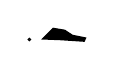
\begin{tikzpicture}[x=.5cm,y=.5cm]\draw (-.3,0) circle (.03);\fill (0,0)--(.3,.3)--(.6,.25)--(.8,.12)--(1.15,.05)--(1.1,-.06)--(.5,-.02)--cycle;\end{tikzpicture}}

\begin{center}$-\ 20\ -$\end{center}\hfill n\textsuperscript{o} 276

\S2. -- \uline{Anneaux} $\mathrm m$-\uline{adiques noethériens}.

Dans tout ce \S\ on désigne par $A$ un anneau \uline{commutatif noethérien} et par $\mathrm m$ un idéal de $A$ ; sauf mention explicite du contraire on munira $A$, et plus généralement tous les $A$-modules considérés, de la topologie $\mathrm m$-adique.

\figure{\begin{tikzpicture}[x=.5cm,y=.5cm]\draw[gray] (0,1) .. controls (-2,1.5) and (-3,-.5) .. (-.5,-.8) .. controls (.3,-.8) and (.7,-.2) .. (1.1,-.1);\draw (1.1,-.1)--(1.5,.05);\draw (2,-.1)--(4,-.1);\draw (2.3,.15)--(4,.15);\draw[gray] (.6,-1.3) circle (.35);\draw[gray] (-.25,-2.3) circle (.38);\end{tikzpicture}}

1. -- \uline{Restriction de la topologie} $\mathrm m$-\uline{adique à un sous-module}.

\uline{Théorème} 1 -- \uline{Soient} $E$ \uline{un} $A$-\uline{module de type fini et} $F$ \uline{un sous-module de} $E$. \uline{La topologie} $\mathrm m$-\uline{adique du} $A$-\uline{module} $F$ \uline{est induite par la topologie} $\mathrm m$-\uline{adique de} $E$.

Le théorème 1 sera une conséquence du résultat plus précis que voici :

\uline{Lemme d'Artin-Rees} \unsure{--} \uline{Soient} $A$ \uline{un anneau commutatif noethérien}, $\mathrm m$ \uline{un idéal de} $A$, $E$ \uline{un} $A$-\uline{module de type fini et} $F$ \uline{un sous-module de} $E$. \uline{Pour tout entier} $k$ \uline{suffisamment grand on a}
\[
\mathrm m^pE\cap F=\mathrm m^{p-k}(\mathrm m^kE\cap F)\qquad\uline{\text{pour tout}}\ p\geq k.
\]
Il suffit évidemment de prouver l'inclusion\qquad --
\[
\mathrm m^pE\cap F\subset\mathrm m^{p-k}(\mathrm m^kE\cap F),
\]
puisque l'inclusion opposée est triviale.

Pour cela considérons dans l'anneau de polynômes $A[X]$ le sous-anneau $A'$ formé des polynômes $\sum a_pX^p$ tels que $a_p\in\mathrm m^p$ pour tout $p$. Il est clair qu'en tant qu'algèbre sur $A$, $A'$ est engendré par les $a_iX$ où $a_i$ est un système de générateurs de $\mathrm m$ ; par suite $A'$ est un anneau noethérien, par ailleurs gradué.

Formons de même le $A[X]$-module
\[
E[X]=A[X]\underset{A}{\otimes}E
\]
des polynômes à coefficients dans $E$ ; en tant que $A'$-module, $E[X]$ contient le sous-module $E'$ formé des polynômes $\sum e_px^p$ tels que $e_p\in\mathrm m^pE$
